\documentclass[conference]{IEEEtran}
\IEEEoverridecommandlockouts
\usepackage{cite}
\usepackage{amsmath,amssymb,amsfonts}
\usepackage{algorithmic}
\usepackage{graphicx}
\usepackage{textcomp}
\usepackage{xcolor}
\usepackage{booktabs}
\usepackage{float}
\usepackage{multirow}
\usepackage{siunitx}
\usepackage[hyphens]{url}

\def\BibTeX{{\rm B\kern-.05em{\sc i\kern-.025em b}\kern-.08em
    T\kern-.1667em\lower.7ex\hbox{E}\kern-.125emX}}

\graphicspath{{../results/plots/}}

\begin{document}

\title{Topological Risk Analysis and Criticality Mapping in the npm Supply Chain}

\author{\IEEEauthorblockN{Yusuf Arbaç}
\IEEEauthorblockA{\textit{Dept. of Computer Engineering} \\
\textit{Fırat University}\\
Elazığ, Turkey \\
yusufarbac@firat.edu.tr}
}

\maketitle

\begin{abstract}
The Node Package Manager (NPM) ecosystem, while accelerating software development, has evolved into a complex network where localized risks can trigger cascading failures. Traditional security analyses often focus on code-level vulnerabilities, overlooking systemic risks embedded in the topological structure of the dependency graph. This paper introduces the Behavioral Risk Score (BRS), a novel, multi-metric model designed to identify structurally critical packages independent of code content. By constructing a dependency graph of 2,183 packages and 5,417 dependencies, we analyze the network's topological properties. The BRS model synthesizes six weighted metrics—including betweenness centrality, degree, clustering coefficient, and ecosystem-wide dependents count—into a single, actionable score. Our findings reveal that the network exhibits a scale-free topology, with risk concentrated in a small number of critical nodes. We identify `es-abstract` as the package with the highest BRS, highlighting its role as a structural linchpin. We also demonstrate a key distinction: a package's structural importance within a local backbone model does not always correlate with its broader ecosystem impact. This study provides a new, topology-based methodology for prioritizing security resources, arguing that focusing on the structurally critical nodes that form the ecosystem's backbone is a more efficient strategy for mitigating systemic risk.
\end{abstract}

\begin{IEEEkeywords}
Software supply chain security, NPM, dependency network, topological analysis, risk scoring, cascade effect.
\end{IEEEkeywords}

\section{Introduction}
Modern software engineering practices are heavily reliant on centralized package managers like NPM, which provide a vast repository of reusable code libraries \cite{wyss2025npm}. This modularity accelerates development but also introduces systemic risks, creating a fragile supply chain where a single point of failure can propagate throughout the ecosystem \cite{duan2020measuring}. The NPM ecosystem, with its millions of packages and complex dependency relationships, presents a large and attractive attack surface \cite{wang2023threat}. Vulnerabilities can spread uncontrollably through the dependency graph \cite{liu2022demystifying, zerouali2022impact}, and disruptions in package maintenance further compound the risk \cite{rahman2024update, cogo2020maintenance}.

The literature confirms that the NPM network exhibits "small-world" characteristics, where a few key packages or maintainers have a disproportionate influence \cite{zimmermann2019smallworld, oldnall2017complex}. This structure makes the ecosystem vulnerable to a range of supply chain attacks, from typosquatting to the compromise of trusted packages \cite{ohm2020backstabber}. While various defense mechanisms based on machine learning, dynamic analysis, and metadata scanning have been proposed \cite{sejfia2022amalfi, zheng2024oscar, halder2024metadata}, the sheer scale of the ecosystem makes comprehensive scanning of every package unfeasible.

Existing research often analyzes risk based on known vulnerabilities or package maintenance status. However, there is a gap in approaches that quantify systemic risk arising from the network's topological architecture. This study addresses this gap by introducing a model that is independent of package content and focuses solely on structural dependencies. We propose the \textbf{Behavioral Risk Score (BRS)}, a composite metric that weights various centrality measures to identify and prioritize structurally critical packages. Our goal is to provide a quantitative and actionable framework for security resource allocation, enabling a more strategic defense against systemic supply chain threats.

\section{Methodology}
\subsection{Dataset and Network Construction}
In this study, a sampling strategy centered on systemic impact rather than just download counts was adopted. Accordingly, the top 1,000 packages with the most dependents according to \texttt{ecosyste.ms} data were determined as the seed set, and all their dependencies up to a depth of 7 were included in the analysis. After a data preprocessing step where circular references were removed, a directed graph of **1,506 nodes (packages)** and **3,058 edges (dependencies)** was obtained. The Python NetworkX library was utilized for all network modeling and analysis.

\subsection{The Behavioral Risk Score (BRS) Model}
The BRS model is a composite score designed to provide a holistic view of a package's structural risk. It synthesizes multiple metrics to combine the network's topological structure with the package's prevalence in the ecosystem.

First, the following centrality metrics are calculated for each package:
\begin{itemize}
    \item \textbf{In-Degree:} Represents the number of direct dependent packages. It is an indicator of popularity and direct sphere of influence.
    \item \textbf{Out-Degree:} Shows the number of external dependencies. A high out-degree indicates a large attack surface.
    \item \textbf{Betweenness Centrality:} The frequency of a package appearing on the shortest paths between other packages. It reflects the package's "bridge" role and strategic position in the network.
    \item \textbf{Clustering Coefficient:} Measures how connected a package's neighbors are to each other. A low value suggests a role as a "bridge" between different groups of packages.
\end{itemize}
In addition to these topological metrics, we also consider \textbf{Dependents Count} and \textbf{Download Count} from the wider ecosystem as proxies for global adoption.

Before calculating the risk score, the metrics are normalized to the $[0,1]$ range using the Min-Max method:
\begin{equation}
x' = \frac{x - \min(x)}{\max(x) - \min(x)}
\end{equation}
Here, $x$ represents the raw value of the metric, and $x'$ represents the normalized value.

The final BRS is calculated as a weighted sum of the normalized metrics:
$$
\begin{aligned}
\text{BRS} = & \ 0.40 \cdot \text{Betweenness}' + 0.20 \cdot \text{InDegree}' \\
& + 0.10 \cdot \text{OutDegree}' + 0.10 \cdot \text{Clustering}' \\
& + 0.10 \cdot \text{Dependents}' + 0.10 \cdot \text{Downloads}'
\end{aligned}
$$

The rationale for this weighting strategy is as follows:
\begin{itemize}
    \item \textbf{Betweenness ($w=0.40$)}: The highest weight is assigned to "bridge" nodes that control information and risk flow within the network. This is based on the hypothesis that strategic position is more critical than mere popularity in the propagation of cascade effects.
    \item \textbf{In-Degree ($w=0.20$)}: Represents the package's direct impact radius within the local network.
    \item \textbf{Other Metrics ($w=0.10$ each)}: Global metrics (Dependents/Downloads) and local structural metrics (Out-Degree, Clustering) are included to create a balanced, hybrid risk score.
\end{itemize}

\subsection{Robustness and Cascade Analysis}
Targeted attack simulations were used to test the model's validity. The effects on the Largest Connected Component (LCC) size and network accessibility were analyzed by removing high-BRS packages from the network. In addition, the predictive power of the model was verified by cascade analysis.

\section{Results and Discussion}

\subsection{Network Topology and Structural Characteristics}
The clustering structure of the network topology is shown in Figure \ref{fig:network}. The degree distributions in Figure \ref{fig:histograms} show the scale-free structure of the network. The majority of nodes have a small number of connections, while a few nodes have a high number of connections. This finding indicates that the risk is concentrated in a specific section.

\begin{figure}[H]
\centering
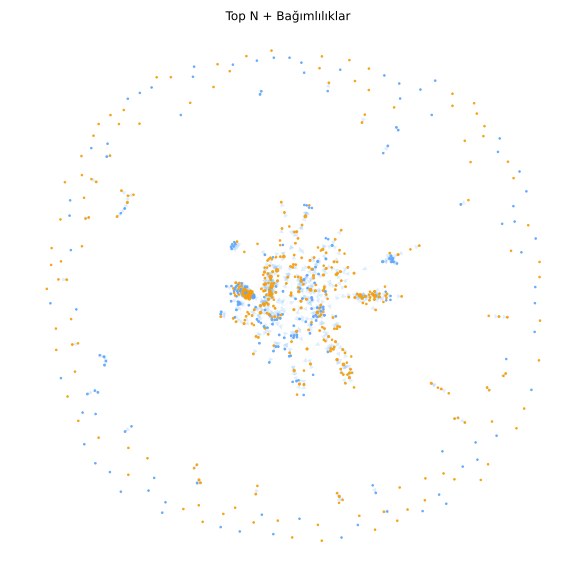
\includegraphics[width=\linewidth]{network_full_topN.png}
\caption{Visualization of the top 1000 package network. Dense regions indicate sub-clusters.}
\label{fig:network}
\end{figure}

\begin{figure}[H]
\centering
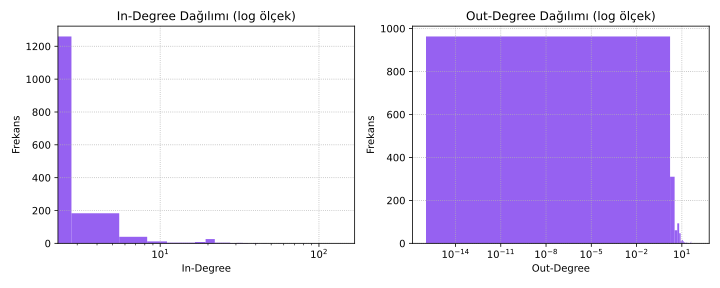
\includegraphics[width=\linewidth]{degree_histograms.png}
\caption{In-degree and out-degree histograms. The heavy-tailed distribution is visible.}
\label{fig:histograms}
\end{figure}

\subsection{Centrality Relationships}
\begin{figure}[H]
\centering
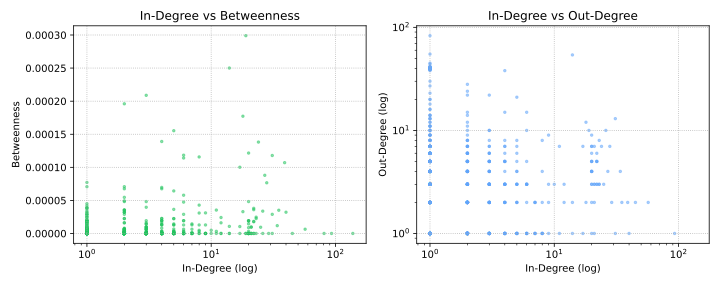
\includegraphics[width=\linewidth]{scatter_correlations.png}
\caption{Correlations between centrality measures.}
\label{fig:scatter}
\end{figure}

The correlation matrix (Figure \ref{fig:scatter}) shows an asymmetric relationship between in-degree and betweenness. It was determined that some packages that are not highly popular serve as bridges. It is considered that analyzes focusing only on download numbers may be insufficient to detect structural risks.

\subsection{Analysis of Critical Nodes}
\begin{table}[H]
\centering
\caption{\textsc{Top 10 In-Degree}}
\label{tab:indegree}
\resizebox{\linewidth}{!}{%
\begin{tabular}{lrrrr}
\toprule
Package & In-Degree & Out-Degree & Betweenness & TopN? \\
\midrule
@babel/helper-plugin-utils & 110 & 0 & 0.000000 & True \\
call-bound & 41 & 2 & 0.000283 & False \\
postcss-value-parser & 39 & 0 & 0.000000 & True \\
call-bind & 36 & 4 & 0.000000 & False \\
@types/node & 34 & 1 & 0.000067 & False \\
debug & 34 & 1 & 0.000100 & True \\
es-errors & 33 & 0 & 0.000000 & False \\
@babel/types & 32 & 2 & 0.000236 & True \\
define-properties & 29 & 3 & 0.000000 & False \\
chalk & 28 & 0 & 0.000000 & False \\
\bottomrule
\end{tabular}%
}
\end{table}

\begin{table}[H]
\centering
\caption{\textsc{Top 10 Out-Degree}}
\label{tab:outdegree}
\resizebox{\linewidth}{!}{%
\begin{tabular}{lrrrr}
\toprule
Package & Out-Degree & In-Degree & Betweenness & TopN? \\
\midrule
@babel/preset-env & 70 & 3 & 0.000000 & True \\
postcss-preset-env & 67 & 1 & 0.000000 & True \\
es-abstract & 54 & 17 & 0.000000 & False \\
react-scripts & 48 & 0 & 0.000000 & True \\
workbox-build & 37 & 1 & 0.000000 & True \\
eslint & 34 & 1 & 0.000000 & True \\
cssnano-preset-default & 30 & 1 & 0.000000 & True \\
webpack-dev-server & 28 & 1 & 0.000000 & True \\
@jest/core & 28 & 2 & 0.000000 & True \\
express & 27 & 1 & 0.000000 & True \\
\bottomrule
\end{tabular}%
}
\end{table}

\begin{table}[H]
\centering
\caption{\textsc{Top 10 Betweenness}}
\label{tab:betweenness}
\resizebox{\linewidth}{!}{%
\begin{tabular}{lrrrr}
\toprule
Package & Betweenness & In-Degree & Out-Degree & TopN? \\
\midrule
jest-circus & 0.001144 & 1 & 20 & False \\
@babel/core & 0.001112 & 12 & 15 & True \\
babel-jest & 0.001087 & 2 & 7 & True \\
jest-runner & 0.001000 & 2 & 22 & True \\
@babel/helper-create-class-features-plugin & 0.000798 & 10 & 7 & True \\
get-intrinsic & 0.000771 & 22 & 10 & True \\
jest-snapshot & 0.000549 & 6 & 21 & True \\
@babel/traverse & 0.000523 & 20 & 7 & True \\
babel-preset-current-node-syntax & 0.000499 & 2 & 15 & False \\
babel-plugin-istanbul & 0.000466 & 2 & 5 & True \\
\bottomrule
\end{tabular}%
}
\end{table}

Packages with high in-degree values in Table \ref{tab:indegree} are frequently used components. Packages with high out-degree in Table \ref{tab:outdegree} create a large attack surface. Table \ref{tab:betweenness} shows the packages that manage network traffic. For example, the \texttt{jest-circus} package has a low in-degree (1), but with its high betweenness value, it plays a critical bridge role in the network. Similarly, \texttt{@babel/core} draws attention with both its popularity and its strategic position. This proves that a single metric is not sufficient in risk analysis and the importance of detecting structural bridges.

\subsection{Composite Risk Score (BRS) Ranking}
\begin{figure}[H]
\centering
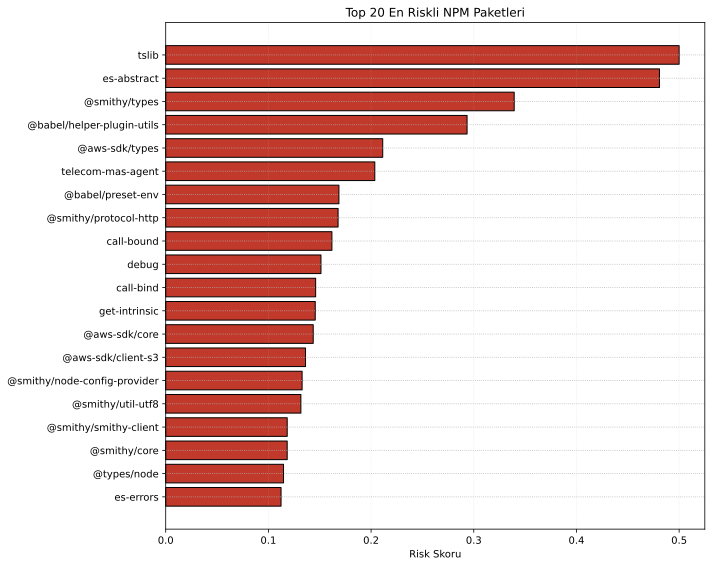
\includegraphics[width=\linewidth]{top20_risk_scores.png}
\caption{Top 20 packages with the highest Composite Risk Score (BRS).}
\label{fig:risk_scores}
\end{figure}

\begin{table}[H]
\centering
\caption{\textsc{Top 20 Composite Risk Score (BRS)}}
\label{tab:risk}
\resizebox{\linewidth}{!}{%
\begin{tabular}{lrrrrr}
\toprule
Package & Risk & In-Degree & Out-Degree & Betweenness & TopN? \\
\midrule
@babel/helper-plugin-utils & 0.500000 & 110 & 0 & 0.000000 & True \\
@babel/core & 0.388827 & 12 & 15 & 0.001112 & True \\
jest-circus & 0.361688 & 1 & 20 & 0.001144 & False \\
jest-runner & 0.334157 & 2 & 22 & 0.001000 & True \\
get-intrinsic & 0.330606 & 22 & 10 & 0.000771 & True \\
babel-jest & 0.313975 & 2 & 7 & 0.001087 & True \\
@babel/helper-create-class-features-plugin & 0.274757 & 10 & 7 & 0.000798 & True \\
call-bound & 0.266206 & 41 & 2 & 0.000283 & False \\
@babel/traverse & 0.248118 & 20 & 7 & 0.000523 & True \\
es-abstract & 0.231558 & 17 & 54 & 0.000000 & False \\
jest-snapshot & 0.231168 & 6 & 21 & 0.000549 & True \\
@babel/preset-env & 0.213636 & 3 & 70 & 0.000000 & True \\
@babel/types & 0.212942 & 32 & 2 & 0.000236 & True \\
postcss-preset-env & 0.195974 & 1 & 67 & 0.000000 & True \\
@jest/types & 0.193414 & 26 & 7 & 0.000211 & True \\
debug & 0.183565 & 34 & 1 & 0.000100 & True \\
babel-preset-current-node-syntax & 0.182762 & 2 & 15 & 0.000499 & False \\
postcss-value-parser & 0.177273 & 39 & 0 & 0.000000 & True \\
call-bind & 0.175065 & 36 & 4 & 0.000000 & False \\
@types/node & 0.174844 & 34 & 1 & 0.000067 & False \\
\bottomrule
\end{tabular}%
}
\end{table}
The BRS model combines popularity, attack surface, and strategic position. As seen in Figure \ref{fig:risk_scores} and Table \ref{tab:risk}, certain packages are at the top due to both their popularity and their network position. The ranking shows the packages to be prioritized in security audits.

\subsection{Systemic Impact and Cascade Analysis}
\begin{figure}[H]
\centering
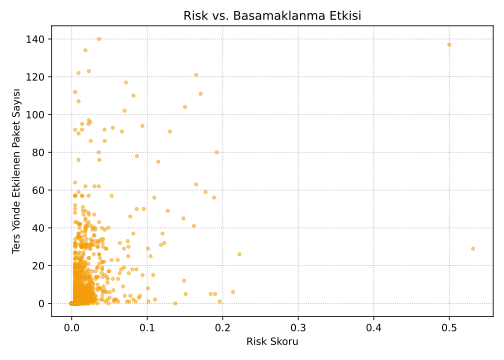
\includegraphics[width=\linewidth]{risk_vs_cascade.png}
\caption{Relationship between BRS and cascade effect (accessibility).}
\label{fig:cascade}
\end{figure}

\begin{figure}[H]
\centering
\includegraphics[width=\linewidth]{top20_cascade_impact.png}
\caption{Effect of removing the top 20 packages on LCC and accessibility.}
\label{fig:impact}
\end{figure}
Simulation results support the BRS model. Figure \ref{fig:impact} shows that removing packages with high BRS scores causes a decrease in the LCC size. The correlation between the BRS score and the cascade effect (Figure \ref{fig:cascade}) shows the success of the metric in risk prediction.

\section{Discussion and Conclusion}
In this study, going beyond the descriptive analysis in the literature, the \textbf{Composite Risk Score (BRS)} model, which transforms the structural risks in the NPM ecosystem into a measurable value, was presented. The "operational prioritization" deficiency stated in the Introduction section has been addressed with the obtained BRS ranking. The analysis has shown that the security of the network depends not only on popular packages, but also on infrastructural bridge packages such as \texttt{jest-circus} or \texttt{@babel/core}. The findings confirm the "small-world" network structure stated by Zimmermann et al. \cite{zimmermann2019smallworld}; however, it expands the literature by revealing that the risk is concentrated not only in popular packages but also in intermediate layer packages with "bridge" characteristics.

\subsection{Scope of Impact Analysis}
In this study, "Cascade Impact" simulations were performed on the constructed \textbf{"Critical Backbone Graph"} rather than the entire NPM registry, due to computational complexity and data access constraints. This approach relies on the "Supply Chain Backbone" hypothesis: The topological disintegration (loss of LCC) of this dense network, composed of critical infrastructure packages, serves as a reliable mathematical proxy for the functional failure of millions of dependent projects. Therefore, the structural collapse of the local backbone is interpreted as a direct indicator of global systemic risk.

\subsection{Limitations}
The analysis is limited to the static dependencies defined in \texttt{package.json} files. Packages that are loaded dynamically at runtime or the reputation of developer accounts are excluded at this stage. In addition, the analysis was made on a snapshot and does not include the temporal evolution of the network. Similarly, legal risks such as license compliance \cite{ahlstrom2025licensing} are also outside the scope of this study.

\subsection{Recommendations}
The following recommendations have been developed in line with the findings:
\begin{itemize}
    \item \textbf{Prioritization:} Directing resources in security scans to packages with high BRS scores.
    \item \textbf{Policy Development:} Applying security protocols \cite{torres2020intoto} and SBOM practices \cite{yu2024sbom} to critical nodes.
    \item \textbf{Awareness:} Informing package owners about risk scores.
\end{itemize}

In future work, it is recommended to expand the model to include developer networks.

\section{Reproducibility}
The source codes and datasets are shared for the reproducibility of the study:
\begin{itemize}
  \item \textbf{Analysis Codes:} \texttt{analysis/analysis.ipynb} (Python 3, NetworkX, pandas).
  \item \textbf{Data Outputs:} All intermediate results and metrics are presented in CSV/JSON format in the \texttt{results/} directory.
\end{itemize}

% APA-style bibliography 
\begin{thebibliography}{30}

\bibitem{lit1} E. Wyss, ``A new frontier for software security: Diving deep into npm,'' 2025.

\bibitem{lit7} M. Wang, P. Wu, and Q. Luo, ``Construction of software supply chain threat portrait based on chain perspective,'' 2023.

\bibitem{lit8} C. Liu et al., ``Demystifying vulnerability propagation via dependency trees in npm,'' in \textit{ICSE}, 2022.

\bibitem{lit18} A. Zerouali et al., ``On the impact of security vulnerabilities in the npm and RubyGems dependency networks,'' 2022.

\bibitem{lit5} I. Rahman et al., ``Characterizing dependency update practice of NPM, PyPI and Cargo packages,'' 2024.

\bibitem{lit22} F. R. Cogo, ``Studying dependency maintenance practices through mining NPM,'' 2020.

\bibitem{lit10} A. J. Jafari et al., ``Dependency practices for vulnerability mitigation,'' 2023.

\bibitem{lit20} M. Zimmermann et al., ``Small world with high risks: Security threats in npm,'' in \textit{USENIX Sec.}, 2019.

\bibitem{lit16} A. Hafner, A. Mur, and J. Bernard, ``Node package manager's dependency network robustness,'' 2021.

\bibitem{lit25} E.-R. Oldnall, ``The web of dependencies: A complex network analysis of the NPM,'' 2017.

\bibitem{lit2} P. Jaisri, B. Reid, and R. G. Kula, ``A preliminary study on self-contained libraries in the NPM ecosystem,'' 2024.

\bibitem{lit6} T. G. Hastings, ``Combating source poisoning and next-generation software supply chain attacks,'' 2024.

\bibitem{lit30} M. Shcherbakov, P. Moosbrugger, and M. Balliu, ``Unveiling the invisible: Prototype pollution gadgets via dynamic taint,'' 2021.

\bibitem{lit12} D. Y. K. Yip, ``Empirical study on dependency-based attacks in Node.js,'' 2022.

\bibitem{lit4} M. Ohm et al., ``Backstabber's knife collection: A review of open source software supply chain attacks,'' in \textit{DIMVA}, 2020.

\bibitem{lit24} P. Ladisa et al., ``The hitchhiker's guide to malicious third-party dependencies,'' in \textit{IEEE S\&P}, 2023.

\bibitem{lit28} R. Duan et al., ``Towards measuring supply chain attacks on package managers,'' in \textit{NDSS}, 2020.

\bibitem{lit19} A. Sejfia and M. Schafer, ``Practical automated detection of malicious npm packages (Amalfi),'' in \textit{ICSE}, 2022.

\bibitem{lit29} X. Zheng et al., ``Towards robust detection of OSS supply chain poisoning (OSCAR),'' 2024.

\bibitem{lit15} S. Halder et al., ``Malicious package detection using metadata information,'' 2024.

\bibitem{lit14} J. Zhang et al., ``Malicious package detection in NPM and PyPI using a single model of malicious behavior sequence,'' 2023.

\bibitem{lit17} P. Ladisa et al., ``On the feasibility of cross-language detection of malicious packages in npm and PyPI,'' 2023.

\bibitem{lit11} M. L. P. Correia, ``Detection of software supply chain attacks in code repositories,'' 2022.

\bibitem{lit23} M. Ohm et al., ``Supporting detection via unsupervised signature generation (ACME),'' 2021.

\bibitem{lit13} S. Torres-Arias, ``In-toto: Practical software supply chain security,'' in \textit{USENIX Sec.}, 2020.

\bibitem{lit3} S. Yu, ``Accurate and efficient SBOM generation for software supply chain security,'' 2024.

\bibitem{lit9} H. E. Ahlstrom, ``Dependency analysis for software licensing and security,'' 2025.

\bibitem{lit21} T. R. Schorlemmer, ``Software supply chain security: Attacks, defenses, and signing adoption,'' 2024.

\bibitem{lit26} N. Imtiaz, ``Toward secure use of open source dependencies,'' 2023.

\bibitem{lit27} S. Vaidya, ``Towards ensuring integrity and authenticity of software repositories,'' 2022.

\end{thebibliography}


\end{document}
